\RequirePackage{plautopatch}
\documentclass[english, dvipdfmx, a4paper]{jsarticle}
\usepackage{docmute}
\usepackage[utf8]{inputenc}
\usepackage[top=10truemm, bottom=20truemm, left=15truemm, right=15truemm]{geometry} % mergin
\renewcommand{\headfont}{\bfseries}

% graphics
\usepackage{graphicx}
\usepackage{here}

% link

\usepackage{url}
\usepackage[dvipdfmx, linktocpage]{hyperref} 
\usepackage{xcolor}
\usepackage{pxjahyper}
\hypersetup{
	colorlinks=true,
	citecolor=blue,
	linkcolor=teal,
	urlcolor=orange,
}

% math

\usepackage{amsmath, amssymb} 
\usepackage{physics}
\usepackage{mathrsfs}
\usepackage{mathtools}

% theoremstyle
\usepackage{amsthm}
\newtheoremstyle{break}
{\topsep}{\topsep}%
{}{}%
{\bfseries}{}%
{\newline}{}%
\theoremstyle{break}
\newtheorem{thm}{Theorem}[section]
\newtheorem{defn}[thm]{Definition}
\newtheorem{eg}[thm]{Example}
\newtheorem{cl}[thm]{Claim}
\newtheorem{cor}[thm]{Corollary}
\newtheorem{fact}[thm]{Fact}
\newtheorem{rem}[thm]{Remark}
\newtheorem{prob}{Problem}[section]
\newtheorem{prop}{Property}

\makeatletter
\newenvironment{pr}[1][\proofnam]{\par
\topsep6\p@\@plus6\p@ \trivlist
\item[\hskip\labelsep{\itshape #1}\@addpunct{\bfseries}]\ignorespaces
}{%
\endtrivlist
}
\newcommand{\proofnam}{\underline{Derivation.}}
\makeatother
% ordinary
	\newcommand{\R}{\mathbb{R}}
	\newcommand{\C}{\mathbb{C}}
	\newcommand{\Z}{\mathbb{Z}}
	
	
	% Physics %%%%%%%%%%%%%%%%%%%%%%%%%%%%%%%%%%%%
	
	% Feynman slash
	\newcommand{\slashed}[1]{#1\!\!\!/}
	% order
	
	%Lie algebra
	\renewcommand{\O}{\mathcal{O}}
	\newcommand{\SO}{\mathrm{SO}}
	\newcommand{\so}{\mathfrak{so}}
	\newcommand{\SU}{\mathrm{SU}}
	\newcommand{\su}{\mathfrak{su}}
	\newcommand{\SP}{\mathrm{SP}}
	\renewcommand{\sp}{\mathfrak{sp}}
	\newcommand{\SL}{\mathrm{SL}}
	\renewcommand{\sl}{\mathfrak{sl}}
	\newcommand{\GL}{\mathrm{GL}}
	\newcommand{\gl}{\mathfrak{gl}}
	\newcommand{\U}{\mathrm{U}}
	\renewcommand{\u}{\mathfrak{u}}
\renewcommand{\i}{\mathrm{i}}
\newcommand{\e}{\mathrm{e}}
\newcommand{\N}{\mathcal{N}}
\newcommand{\Q}{\mathcal{Q}}
\renewcommand{\P}{\mathcal{P}}
\renewcommand{\S}{\text{S}}
% number

\makeatletter
\@addtoreset{equation}{section}
\makeatother
\numberwithin{equation}{section}
\renewcommand{\thefootnote}{\roman{footnote}.}
\renewcommand{\appendixname}{Appendix }

\title{SUSYQM}
\author{Toshiya Tanaka}
\date{\today}

\begin{document}
	\maketitle
	\documentclass[english, dvipdfmx, a4paper]{jsarticle}
\usepackage[utf8]{inputenc}
\usepackage[top=10truemm, bottom=20truemm, left=15truemm, right=15truemm]{geometry} % mergin
\renewcommand{\headfont}{\bfseries}

% graphics
\usepackage{graphicx}
\usepackage{here}

% link

\usepackage{url}
\usepackage[dvipdfmx, linktocpage]{hyperref} 
\usepackage{xcolor}
\usepackage{pxjahyper}
\hypersetup{
	colorlinks=true,
	citecolor=blue,
	linkcolor=teal,
	urlcolor=orange,
}

% math

\usepackage{amsmath, amssymb} 
\usepackage{physics}
\usepackage{mathrsfs}
\usepackage{mathtools}

% theoremstyle
\usepackage{amsthm}
\newtheoremstyle{break}
{\topsep}{\topsep}%
{}{}%
{\bfseries}{}%
{\newline}{}%
\theoremstyle{break}
\newtheorem{thm}{Theorem}[section]
\newtheorem{defn}[thm]{Definition}
\newtheorem{eg}[thm]{Example}
\newtheorem{cl}[thm]{Claim}
\newtheorem{cor}[thm]{Corollary}
\newtheorem{fact}[thm]{Fact}
\newtheorem{rem}[thm]{Remark}
\newtheorem{prop}{Property}
\newtheorem{prob}{Problem}[section]

\makeatletter
\newenvironment{pr}[1][\proofnam]{\par
\topsep6\p@\@plus6\p@ \trivlist
\item[\hskip\labelsep{\itshape #1}\@addpunct{\bfseries}]\ignorespaces
}{%
\endtrivlist
}
\newcommand{\proofnam}{\underline{Derivation.}}
\makeatother
\renewcommand{\i}{\mathrm{i}}
\newcommand{\e}{\mathrm{e}}
\newcommand{\N}{\mathcal{N}}

% number

%\makeatletter
%\@addtoreset{equation}{section}
%\makeatother
%\numberwithin{equation}{section}
%\renewcommand{\thefootnote}{\roman{footnote}.}
%\renewcommand{\appendixname}{Appendix }
\title{}
\author{Toshiya Tanaka}
\date{\today}

\begin{document}
	\section{SUSY in QM}
	\begin{defn}[最小超対称関係]
		3種類のHermitian operator $H$: Hamiltonian, $Q$: Supercharge, $(-1)^F$: ???があって
		\begin{align}
			H &= Q^2\\
			Q(-1)^{F} &= -(-1)^{F}Q,\quad  \text{or}\quad \{Q, (-1)^F\} =0\\
			\qty((-1)^{F})^2 &=1
		\end{align}
		を満たす関係を最小超対称関係という.

		超対称性がある系には,必ずこの関係がある.
	\end{defn}
	実は,簡単な量子力学系にもこの構造が隠れている.
	\subsection{円周上の自由粒子}
	半径$R$の円周上の自由粒子を考える.定義域を$-\pi R\leq x\leq \pi R$とし,
	周期的境界条件$\psi(x+2\pi R) = \psi(x)$を入れる.
	Hamiltonianは$H=-1/(2m)\dv*{}{x}$であるので,Schr\"{o}dinger方程式を解くと,固有関数として,次の固有関数を得る.
	\begin{align}
		\phi_{n,+}(x) &= N_{n,+}\cos\qty(\frac{n}{R}x)\\
		\phi_{n,-}(x) &= N_{n, -} \sin\qty(\frac{n}{R}x).
	\end{align}
	これらの固有エネルギーは,
	\begin{equation}
		E=\frac{1}{2mR^2}n^2
	\end{equation}
	で,各固有空間は$2$次元あることがわかる.Hamiltonianを``因数分解''してsuperchargeを得る.
	$H = (-\i/(\sqrt{2m})\dv*{}{x})^2$より,$Q\coloneqq-\i/(\sqrt{2m})\dv*{}{x}=p/\sqrt{2m}$とする.

	また,parity $\mathcal{P}$は$(-1)^{F}$の働きをする.

	よって,この系には,最小超対称関係を満たす演算子たちが存在することがわかる.
	これらはHermitianであることも確かめられる\footnote{$A$がHermitianとは,
	今定まっている内積$\langle\psi, \phi\rangle=\int\dd{x}\qty(\psi(x))^*\phi(x)$に対して,$\langle A\psi, \phi\rangle = \langle \psi , A\phi\rangle$が成り立つことである.}.

	今,周期的境界条件で考えたが,ひねった境界条件$\psi(x+2\pi R) = \e^{\i\theta}\psi(x)$を入れると面白い\footnote{Aharanov--Bohmのように,磁場を使うと,実際に作ることができる.}.
	$\theta$の連続変形でスペクトラムの構造は連続的に変化し
	\footnote{spectral flowという.},$\theta = n\pi$のところではSUSYの構造が現れるが,その他のところでは現れない.
	実際計算すると,固有エネルギーと固有状態は
	\begin{align}
		\psi_n &= N_{n}\e^{\i(n+\theta/(2\pi))x/R}\\
		E_n &= \frac{1}{2mR^2}\qty(n+\frac{\theta}{2\pi})^2
	\end{align}
	となる.

	$\theta \neq n\pi$でSUSYが壊れているのは,parityが上手くいっていないからである.
	境界条件を考えると,$\psi(x+2\pi R) = \e^{\i\theta}\psi(x)$だが,
	$x' = -x-2\pi R$とおくと,$\psi(x'+2\pi R)=\e^{-\i\theta}\psi(x')$となって
	しまい,$\theta\neq n\pi$ではparityで境界条件が不変でないので,同じ系の中で対応が作れない.
	\subsection{超対称性の基本性質}

	SUSYがある系は最小超対称関係
	\begin{itemize}
		\item $H=Q^2$
		\item $\qty{Q, (-1)^{F}}=0$
		\item $\qty((-1)^{F})=1$
	\end{itemize}
	が必ずある.

	この関係から,$[H, Q]=0$, $[H, (-1)^F]$がなりたつので,$H$と$(-1)^{F}$の
	同時固有状態$\ket{E, \lambda}$をとることができる.$\qty((-1)^{F})^2=1$
	なので,$\lambda = \pm1$である.



	以下の4つの性質が成り立つ.
	\begin{prop}
		エネルギー固有値が非負.$E\geq0$.
	\end{prop}
	次の式変形からわかる\footnote{$Q$がHermitianであることは本質的である.}.
	\begin{align}
		E &= \mel{E, \lambda}{H}{E, \lambda}\\
		  &= \mel{E, \lambda}{Q^2}{E, \lambda}\\
		  &= \|Q\ket{E, \lambda}\|^2\\
		  &\geq0.
	\end{align}\qed
	\begin{prop}
		正エネルギー状態は,$(-1)^{F}$の固有値が$\pm1$の固有状態$\ket{E, \pm}$で対を成し,エネルギー固有値は縮退する.
	\end{prop}
	まず,$E>0$として,$\ket{E, +}$を考える.
	$(-1)^{F}Q\ket{E, +} = -Q(-1)^{F}\ket{E, +} = -Q\ket{E, +}$なので,$Q\ket{E, +}\propto\ket{E, -}$.
	$\ket{E, -}$についても同様にして,$Q\ket{E, -}\propto\ket{E, +}$である.

	また,比例定数は	
	\begin{align}
		\|Q\ket{E,+}\|^2 &= \mel{E, +}{Q^{\dag}Q}{E, +}\\
						 &= \expval{H}{E, +}\\
						 &= E
	\end{align}
	となるので\footnote{phaseは実にとると},
	\begin{equation}
		Q\ket{E,\pm} = \sqrt{E}\ket{E, \mp}\label{eq:normalization}
	\end{equation}
	と決まる\footnote{$Q$は$H$を``因数分解''して作ったことを思い出すと,大きさは$\sqrt{E}$になると思える.}.
	
	このとき,$\ket{E, \pm}$は$Q$を通じて対を成しており,supermultipletを成すという.
	この状況を模式的に$\ket{E, +}\overset{Q}{\longleftrightarrow}\ket{E, -}$と書く.\qed

	\begin{prop}
		ゼロエネルギー状態\footnote{SUSYの文脈でこのような状態をBPS stateという.}は必ずしも縮退しない.
		ゼロエネルギー状態が存在するならば,$Q\ket{E=0}=0$を満たす.
	\end{prop}
	Eq. \eqref{eq:normalization}に$E=0$を代入すると直ちにわかる.
	$E\neq0$のときとは異なり,$Q$を通じたsupermultipletをなさない.
	この状況を$\ket{E=0, +}\overset{Q}{\longrightarrow} 0 \overset{Q}{\longleftarrow} \ket{E=0, -}$と書く.\qed

	ゼロエネルギー状態が$Q\ket{E=0, \pm}$を満たすことは,ゼロエネルギー状態は1階の微分方程式の解であることを意味する.


	\begin{prop}
		Witten index $\Delta_{\text{W}} \coloneqq \N_{E=0}^{+}-\N_{E=0}^{-}$はtopological invariant.

		ここで,$\N_{E=0}^{\pm}$は$(-1)^F$の固有値が$\pm1$の固有状態の数である.
	\end{prop}
	topological invariantとは,理論のパラメータの連続変形で不変な量という意味で用いる.
	$S^1$上の自由粒子の例では$m$や$R$を大きくとると,$n\neq0$に置いても$E_n\to0$となるが,
	もともとnon zeroであるものは対で存在するので,ゼロエネルギー状態の数の差は変わらない.\qed
\end{document}

	\documentclass[english, dvipdfmx, a4paper]{jsarticle}
\usepackage{docmute}
\usepackage[utf8]{inputenc}
\usepackage[top=10truemm, bottom=20truemm, left=15truemm, right=15truemm]{geometry} % mergin
\renewcommand{\headfont}{\bfseries}

% graphics
\usepackage{graphicx}
\usepackage{here}

% link

\usepackage{url}
\usepackage[dvipdfmx, linktocpage]{hyperref} 
\usepackage{xcolor}
\usepackage{pxjahyper}
\hypersetup{
	colorlinks=true,
	citecolor=blue,
	linkcolor=teal,
	urlcolor=orange,
}

% math

\usepackage{amsmath, amssymb} 
\usepackage{physics}
\usepackage{mathrsfs}
\usepackage{mathtools}

% theoremstyle
\usepackage{amsthm}
\newtheoremstyle{break}
{\topsep}{\topsep}%
{}{}%
{\bfseries}{}%
{\newline}{}%
\theoremstyle{break}
\newtheorem{thm}{Theorem}[section]
\newtheorem{defn}[thm]{Definition}
\newtheorem{eg}[thm]{Example}
\newtheorem{cl}[thm]{Claim}
\newtheorem{cor}[thm]{Corollary}
\newtheorem{fact}[thm]{Fact}
\newtheorem{rem}[thm]{Remark}
\newtheorem{prob}{Problem}[section]
\newtheorem{prop}{Property}

\makeatletter
\newenvironment{pr}[1][\proofnam]{\par
\topsep6\p@\@plus6\p@ \trivlist
\item[\hskip\labelsep{\itshape #1}\@addpunct{\bfseries}]\ignorespaces
}{%
\endtrivlist
}
\newcommand{\proofnam}{\underline{Derivation.}}
\makeatother
\newcommand{\Z}{\mathbb{Z}}
\newcommand{\C}{\mathbb{C}}
\renewcommand{\i}{\mathrm{i}}
\newcommand{\e}{\mathrm{e}}
\newcommand{\N}{\mathcal{N}}
\newcommand{\Q}{\mathcal{Q}}
\renewcommand{\P}{\mathcal{P}}
% number

%\makeatletter
%\@addtoreset{equation}{section}
%\makeatother
%\numberwithin{equation}{section}
%\renewcommand{\thefootnote}{\roman{footnote}.}
%\renewcommand{\appendixname}{Appendix }

\title{SUSYQM}
\author{Toshiya Tanaka}
\date{\today}

\begin{document}
\section{\texorpdfstring{$\N=2$}{N=2}超対称代数}
	\subsection{一般性質}
	\begin{defn}[実superchargeと$\N = 2$\footnote{$\N$はsuperchargeの数である.ところが,実(エルミート)で数える流儀と複素で数える流儀があり,文献を比較する際は確認する必要がある.今は実で数えている.}超対称代数]
		最小超対称関係を満たす三つのエルミート演算子$H$, $Q$, $(-1)^{F}$から,
		エルミート演算子\footnote{エルミートという意味で,実superchargeという.}
		$Q_1 \coloneqq Q$, $Q_2\coloneqq -\i Q(-1)^{F}$
		を定める.
		$H$, $Q_1$, $Q_2$は,		\begin{align}
			\qty{Q_i, Q_j} &= 2H\delta_{ij}\\
			\qty[H, Q_i] &= 0
		\end{align}
		の関係を満たす.
	\end{defn}
	これは,最小超対称関係と等価だが,$(-1)^{F}$を加えて議論することが多い.
	$(-1)^{F}$は余分な演算子なので,束縛関係$\i Q_1Q_2 = H(-1)^F$で結ばれる\footnote{$(-1)^{F}$という余分な演算子が現れたとき,$H$をかければ最小限の$Q_1$, $Q_2$のみで書けるということ.}.
	\begin{defn}[複素superchargeと$\N = 2$超対称代数]
		$\Q \coloneqq (Q_1 + \i Q_2)/\sqrt{2}$を定める.このとき,$\Q$, $H$は
		\begin{align}
			\qty{\Q^{\dag}, \Q} &= 2H\\
			\qty{\Q, \Q} = \qty{\Q^{\dag}, \Q^{\dag}} &= 0 \label{eq:nilp}\\
			\qty[H, \Q] = \qty[H, \Q^{\dag}] &= 0
		\end{align}
		の関係を満たす.
	\end{defn}
	Eq. \eqref{eq:nilp}は$\Q^2 = (\Q^{\dag})^2 = 0$と書け,$2$乗してゼロになるこの性質をnilpotencyという
	\footnote{nilpotencyは場の理論のGlassmann数の対称性であるBRS対称性による保存量であるBRS charge, de Rham coholomogyなどでも重要な働きをするそう.実際SUSYQMで微分幾何をやるという話もある.}.
	
	複素の場合も,$\N = 2$超対称代数に$(-1)^F$を加え考えることが便利である.
	この場合の束縛関係は
	$\qty(\Q^{\dag}\Q - \Q\Q^{\dag})/2 = H(-1)^{F}$である.左辺を実superchargeで計算すれば,$iQ_1Q_2$になり,実の場合の束縛を使うと導ける.

	複素superchargeで基本性質を見る.
	\setcounter{prop}{0}
	\begin{prop}
		$E\geq0$.
	\end{prop}
	\begin{prop}
		$E>0$なら次のsupermultipletの構造がある.
		\begin{equation}
			0\xleftarrow[\Q]{}\ket{E, -}\xleftrightarrow[\Q]{\Q^{\dag}}\ket{E, +} \xrightarrow[]{\Q^{\dag}} 0\label{eq:positive_spectrum}
		\end{equation}
	\end{prop}
	\begin{prop}
		$E=0$なら,$\Q$, $\Q^{\dag}$で消える.
		\begin{equation}
			0 \xleftarrow[\Q]{}\ket{E=0}\xrightarrow[]{\Q^{\dag}}0\label{eq:zero_spectrum}
		\end{equation}
	\end{prop}
	\begin{prop}
		Witten indexがトポロジカルな量.
	\end{prop}
	Witten indexについては全く同じ.
	\subsection{\texorpdfstring{$S^1$}{S1}上自由粒子での具体例}
	以下では,上で見た$\N=2$超対称代数を,具体的に$S^1$上の自由粒子の例について見る.


	前回,この系は$H\coloneqq -1/(2m)\dv*[2]{}{x}$, $Q\coloneqq -\i/(2m)\dv*{}{x}$, $(-1)^{F}\coloneqq \mathcal{P}$が最小超対称関係を満たすことを見たが,もう少し具体的に見る.

	この系では,周期的境界条件から,エネルギーは$E_n = n^2/(2mR^2),\ n\in\Z_{\geq0}$で対応する固有状態は二つあり,
	\begin{align}
		\psi_{n, +}(x) &= N_{n, +}\cos(nx/R)\quad n\in\Z_{\geq 0}\\
		\psi_{n, -}(x) &= N_{n, -}\sin(nx/R)\quad n \in \Z_{>0}
	\end{align}
	であるが,これは,$Q$が一階微分演算子であり,
	$\sin$と$\cos$が入れ替わることを考えると,$Q$を通して移り合う.

	また,規格化定数のphaseを$N_{n, -} = \i N_{n, +} \eqqcolon \i N_n$ととると,
	\begin{align}
		Q\psi_{n, +} &= \sqrt{n^2/(2mR^2)}\i N_n\sin(nx/R)\\
					 &= \sqrt{E_n}\psi_{n, -}
	\end{align}
	と規格化定数も含めて,一般の結果が再現できる.

	次に,複素superchargeを用いて考える.以下では,具体的な微分などは考えず,
	$H$と$\Q$と$\mathcal{P}$の代数的性質を用いて考察する.

	今,$\P_{\pm}\coloneqq (1 \pm \P)/2$を定めると,
	複素superchargeは$\Q = (Q + \i(-\i Q \mathcal{P}))/\sqrt{2}=\sqrt{2}Q/\P_+$, $\Q^{\dag} = \sqrt{2}Q\P_-$となる.
	
	\begin{thm}
		$\P_{+}$, $\P_{-}$はそれぞれ関数$f(x)$の偶関数成分,奇関数成分を取り出す演算子である.
	\end{thm}
	$f(x) = (f(x) + f(-x))/2 + (f(x) - f(-x))/2$と書き直したとき,第一項は偶関数であり,
	第二項は奇関数である.これらを偶関数成分,奇関数成分と呼ぶ.

	$\P_{\pm}(f(x)) = (f(x) \pm f(-x))/2$は実際に成り立つ.\qed
	\begin{thm}
		$\P_{\pm}$は射影演算子である.すなわち,次の性質を満たす.
		\begin{itemize}
			\item $(\P_{\pm})^2 = \P_{\pm}$
			\item $\P_+ + \P_- = 1$
			\item $\P_+\P_- = 0$
		\end{itemize}
	\end{thm}

	これを用いて,Eq. \eqref{eq:positive_spectrum}のスペクトラムは理解できる.
	\begin{itemize}
		\item $\psi_{n, +}$は偶関数なので,$\Q^{\dag}\sim\P_-$で消える.
		\item $\psi_{n, -}$は奇関数なので,$\Q\sim\P_+$で消える.
		\item $\psi_{n, +}$は偶関数なので,$\Q\sim Q$で奇関数に移る.
		\item $\psi_{n, -}$は奇関数なので,$\Q^{\dag}\sim Q$で偶関数に移る.
	\end{itemize}

	また, Eq. \eqref{eq:zero_spectrum}のスペクトラムは次のように理解できる.
	\begin{itemize}
		\item ground stateは定数関数なので,微分で消える.
		\item 偶関数でもあるので,$\P_-$でも消える.
	\end{itemize}
\end{document}

	\documentclass[english, dvipdfmx, a4paper]{jsarticle}
\usepackage{docmute}
\usepackage[utf8]{inputenc}
\usepackage[top=10truemm, bottom=20truemm, left=15truemm, right=15truemm]{geometry} % mergin
\renewcommand{\headfont}{\bfseries}

% graphics
\usepackage{graphicx}
\usepackage{here}

% link

\usepackage{url}
\usepackage[dvipdfmx, linktocpage]{hyperref} 
\usepackage{xcolor}
\usepackage{pxjahyper}
\hypersetup{
	colorlinks=true,
	citecolor=blue,
	linkcolor=teal,
	urlcolor=orange,
}

% math

\usepackage{amsmath, amssymb} 
\usepackage{physics}
\usepackage{mathrsfs}
\usepackage{mathtools}

% theoremstyle
\usepackage{amsthm}
\newtheoremstyle{break}
{\topsep}{\topsep}%
{}{}%
{\bfseries}{}%
{\newline}{}%
\theoremstyle{break}
\newtheorem{thm}{Theorem}[section]
\newtheorem{defn}[thm]{Definition}
\newtheorem{eg}[thm]{Example}
\newtheorem{cl}[thm]{Claim}
\newtheorem{cor}[thm]{Corollary}
\newtheorem{fact}[thm]{Fact}
\newtheorem{rem}[thm]{Remark}
\newtheorem{prob}{Problem}[section]
\newtheorem{prop}{Property}

\makeatletter
\newenvironment{pr}[1][\proofnam]{\par
\topsep6\p@\@plus6\p@ \trivlist
\item[\hskip\labelsep{\itshape #1}\@addpunct{\bfseries}]\ignorespaces
}{%
\endtrivlist
}
\newcommand{\proofnam}{\underline{Derivation.}}
\makeatother
% ordinary
	\newcommand{\R}{\mathbb{R}}
	\newcommand{\C}{\mathbb{C}}
	\newcommand{\Z}{\mathbb{Z}}
	
	
	% Physics %%%%%%%%%%%%%%%%%%%%%%%%%%%%%%%%%%%%
	
	% Feynman slash
	\newcommand{\slashed}[1]{#1\!\!\!/}
	% order
	
	%Lie algebra
	\renewcommand{\O}{\mathcal{O}}
	\newcommand{\SO}{\mathrm{SO}}
	\newcommand{\so}{\mathfrak{so}}
	\newcommand{\SU}{\mathrm{SU}}
	\newcommand{\su}{\mathfrak{su}}
	\newcommand{\SP}{\mathrm{SP}}
	\renewcommand{\sp}{\mathfrak{sp}}
	\newcommand{\SL}{\mathrm{SL}}
	\renewcommand{\sl}{\mathfrak{sl}}
	\newcommand{\GL}{\mathrm{GL}}
	\newcommand{\gl}{\mathfrak{gl}}
	\newcommand{\U}{\mathrm{U}}
	\renewcommand{\u}{\mathfrak{u}}
\renewcommand{\i}{\mathrm{i}}
\newcommand{\e}{\mathrm{e}}
\newcommand{\N}{\mathcal{N}}
\newcommand{\Q}{\mathcal{Q}}
\renewcommand{\P}{\mathcal{P}}
% number

%\makeatletter
%\@addtoreset{equation}{section}
%\makeatother
%\numberwithin{equation}{section}
%\renewcommand{\thefootnote}{\roman{footnote}.}
%\renewcommand{\appendixname}{Appendix }

\title{SUSYQM}
\author{Toshiya Tanaka}
\date{\today}

\begin{document}
	\section{Witten model}
	\begin{defn}[Witten model]
		Hamiltonianを2成分で
		\begin{equation}
			H = \mqty(A^{\dag}A & 0 \\ 0 & AA^{\dag}) = \mqty(H_+ & 0 \\ 0 & H_-)
		\end{equation}
		の形で与える量子力学系をWitten modelや$\N = 2$超対称量子力学($\N = 2$ SUSYQM)という.量子力学なので,具体的に$A$は
		\begin{equation}
			A \coloneqq \frac{1}{\sqrt{2m}}\qty(-\i\hbar\dv[2]{}{x} - \i W'(x))
		\end{equation}
		と書け,$W(x)$はsuperpotential\footnote{$W'(x)$のことをsuperpotentialという流儀もあって,実際Wittenの原論文はそうだが,$W(x)$のほうがふさわしいらしい.}という.
		また,
		\begin{align}
			H_+ &= \frac{-\hbar^2}{2m}\dv[2]{}{x} + \frac{1}{2m}\qty(W'(x))^2 - \frac{\hbar}{2m}W''(x)\\
			H_- &= \frac{-\hbar^2}{2m}\dv[2]{}{x} + \frac{1}{2m}\qty(W'(x))^2 + \frac{\hbar}{2m}W''(x)
		\end{align}
		である.
		これに伴い,波動関数は二成分考える必要があり,$\Psi(x) = (\psi_+(x), \psi_-(x))^{\top}$と書く.
	\end{defn}

	Witten modelは定義した$H$に加え,
	\begin{equation}
		Q \coloneqq \mqty(0 & A^\dag \\ A & 0), \quad (-1)^{F} = \mqty(1 & 0\\ 0 & -1)
	\end{equation}
	を定めると,これらは最小超対称関係を満たす.

	これから定義に従って計算すると,実superchargeは
	\begin{equation}
		Q_1 = \mqty(0 & A^\dag \\ A & 0), \quad Q_2 = \mqty(0 & \i A^\dag \\ -\i A & 0),
	\end{equation}
	複素superchargeは
	\begin{align}
		\Q &= \mqty(0 & 0 \\ \sqrt{2}A) = \sqrt{2}A\sigma_-\\
		\Q^{\dag} &=\mqty(0 & \sqrt{2}A^{\dag} \\ 0 & 0) = \sqrt{2}A^{\dag}\sigma_+
	\end{align}
	となる.$\sigma_{\pm}$は冪零行列なので,複素superchargeの冪零性はここから
	自然にわかる.

	エネルギーの縮退の構造に関して,今までどおり,$H$と$(-1)^{F}$の同時固有状態を考える.
	$(-1)^{F} = \sigma_3$の形から,固有状態は$(\psi_+(x), 0)^{\top}$, $(0, \psi_-(x))^{\top}$であり,$H\Psi_E(x) = E\Psi_E(x)$は
	\begin{align}
		A^{\dag}A\psi_{E, +}(x) &= E \psi_{E, +}(x)\\
		AA^{\dag}\psi_{E, -}(x) &= E\psi_{E, -}(x)
	\end{align}
	を解けば良いことになる.

	\begin{thm}
		ここで,$E > 0$の場合
		\begin{align}
			A\psi_{E, +}(x) &= \sqrt{E} \psi_{E, -}(x),\label{eq:annihilate}\\
			A^{\dag}\psi_{E, -}(x) &= \sqrt{E}\psi_{E, +}\label{eq:create}
		\end{align}
			の超対称関係がある.
	\end{thm}
	今,Eq. \eqref{eq:annihilate}の一つの解$\psi_{E, +}(x)$を取って,$A\psi_{E, +}(x)$を考えると,
	$AA^{\dag}(A\psi_{E, +})(x)  = EA\psi_{E, +}(x)$よりEq. \eqref{eq:create}の解になる.規格化は$\|A\psi_{E, +}\|^2 = \langle \psi_{E, +}, A^{\dag}A\psi_{E, +}\rangle = E$なので$A\psi_{E, +}(x) = \sqrt{E}\psi_{E, -}(x)$である.もうひとつも同様.\qed

	Witten modelは二成分で考えているが,別個の2つの量子力学系$H_+=A^{\dag}A$, $H_-=AA^{\dag}$を二つ取ってきたと思うと,その間に$A$と$A^{\dag}$を通して
	対応がついたことになる.$H_+$と$H_-$を超対称パートナーHamiltonianという.


	Witten modelのゼロエネルギー状態を調べると,Witten indexに幾何的解釈をつける
	ことができる.
	ゼロエネルギー状態は他とは異なり,一階の微分方程式の解になっている.
	$A\psi_{0, +}(x) = 0 $, $A^{\dag}\psi_{E, -}(x) = 0$だが,微分を明らかに書くと,
	\begin{align}
		\frac{-\i\hbar}{\sqrt{2m}}\qty(\dv{}{x}+\frac{1}{\hbar}W'(x))\psi_{0, +}(x) &= 0\\
		\frac{-\i\hbar}{\sqrt{2m}}\qty(\dv{}{x}-\frac{1}{\hbar}W'(x))\psi_{0, -}(x) &= 0
	\end{align}
	なので,簡単に解けて,
	\begin{align}
		\psi_{0, +}(x) &= N_{0, +}\e^{-W(x)/\hbar}\\
		\psi_{0, -}(x) &= N_{0, -}\e^{W(x)/\hbar}
	\end{align}
	となる.$N_{0, \pm}$は適当な規格化定数である.
	ただし,量子力学としては,この解であり規格化可能なものだけが
	取りうる状態なので規格化可能性を調べる必要がある.

	便宜上,superpotentialが$p$次多項式で$W(x) = a_0 + a_1x + a_2x^2 +\cdots + a_px^{p}$, $a_p\neq 0$で与えられるとする.規格化可能性を考えると,ゼロエネルギー状態はあるとしたらsuperpotentialの最高次が偶数次の場合で,符号が正なら$(-1)^{F}$の固有値が$+1$の方に存在し,負なら$-1$の方に存在することになる.\ref{tab:normalizability}.
	\begin{table}[htbp]
		\centering
		\label{tab:normalizability}
		\caption{$\checkmark$の入っている場合が規格化可能.}
		\begin{tabular}{c | cccc}\hline
			 & $W(\infty)$ & $W(-\infty)$ & $\psi_{0, +}$ & $\psi_{0, -}$\\\hline
			$a_p > 0$, $p$: even & $\infty$ & $\infty$ & $\checkmark$ & $\times$\\
			$a_p > 0$, $p$: odd & $\infty$ & $-\infty$ & $\times$ & $\times$\\
			$a_p < 0$, $p$: even & $-\infty$ & $\infty$ & $\times$ & $\checkmark$\\
			$a_p < 0$, $p$: odd & $-\infty$ & $-\infty$ & $\times$ & $\times$\\\hline
		\end{tabular}
	\end{table}

	Witten indexは
	\begin{equation}
		\Delta_{\text{W}} = 
		\begin{cases}
			+1,\quad & a_p>0, p:\text{ even}\\
			-1,\quad & a_p<0, p:\text{ even}\\
			0, \quad & p:\text{ odd}
		\end{cases}
	\end{equation}
	だが,これはsuperpotentialの$(\text{二回微分が正の極値の数}) - (\text{負の極値の数})$に等しいことが知られている\footnote{Witten1981に書いてあるらしいが,見つけられなかった.}.
	感覚的には,superpotentialを連続変形しても漸近的振る舞いを変えない限り,この数が変わらないこととしてWitten indexがtopological不変量であることが理解できる.


	現象論にもWitten indexは重要で,
	現状,SUSYは現実世界で観測されていないので,low energyではSUSYは破れていないといけない.

	ground state $\ket{\text{vac}}$として,$\Q\ket{\text{vac}} = \Q^{\dag}\ket{\text{vac}} = 0$のときSUSYは破れていない,そうでないときSUSYは破れているという.
	エネルギーの言葉ではこれはground energy $E_0 = 0$のときSUSYが破れている,そうでないときSUSYが破れていないことになる.

	Witten indexの言葉では,$\Delta_\text{W}\neq0$なら,かならずゼロエネルギー状態
	があるので,SUSYは破れていない.
	SUSYが破れているならば,$\Delta_\text{W} = 0$である.(逆は成り立たない.)

	SUSYが破れている現象論模型を作るためには,$\Delta_{\text{W}} = 0$を満たすように作らなければいけない.
\end{document}

	\documentclass[english, dvipdfmx, a4paper]{jsarticle}
\usepackage{docmute}
\usepackage[utf8]{inputenc}
\usepackage[top=10truemm, bottom=20truemm, left=15truemm, right=15truemm]{geometry} % mergin
\renewcommand{\headfont}{\bfseries}

% graphics
\usepackage{graphicx}
\usepackage{here}

% link

\usepackage{url}
\usepackage[dvipdfmx, linktocpage]{hyperref} 
\usepackage{xcolor}
\usepackage{pxjahyper}
\hypersetup{
	colorlinks=true,
	citecolor=blue,
	linkcolor=teal,
	urlcolor=orange,
}

% math

\usepackage{amsmath, amssymb} 
\usepackage{physics}
\usepackage{mathrsfs}
\usepackage{mathtools}

% theoremstyle
\usepackage{amsthm}
\newtheoremstyle{break}
{\topsep}{\topsep}%
{}{}%
{\bfseries}{}%
{\newline}{}%
\theoremstyle{break}
\newtheorem{thm}{Theorem}
\newtheorem{defn}[thm]{Definition}
\newtheorem{eg}[thm]{Example}
\newtheorem{cl}[thm]{Claim}
\newtheorem{cor}[thm]{Corollary}
\newtheorem{fact}[thm]{Fact}
\newtheorem{rem}[thm]{Remark}
\newtheorem{prob}{Problem}
\newtheorem{prop}{Property}

\makeatletter
\newenvironment{pr}[1][\proofnam]{\par
\topsep6\p@\@plus6\p@ \trivlist
\item[\hskip\labelsep{\itshape #1}\@addpunct{\bfseries}]\ignorespaces
}{%
\endtrivlist
}
\newcommand{\proofnam}{\underline{Derivation.}}
\makeatother
% ordinary
	\newcommand{\R}{\mathbb{R}}
	\newcommand{\C}{\mathbb{C}}
	\newcommand{\Z}{\mathbb{Z}}
	
	
	% Physics %%%%%%%%%%%%%%%%%%%%%%%%%%%%%%%%%%%%
	
	% Feynman slash
	\newcommand{\slashed}[1]{#1\!\!\!/}
	% order
	
	%Lie algebra
	\renewcommand{\O}{\mathcal{O}}
	\newcommand{\SO}{\mathrm{SO}}
	\newcommand{\so}{\mathfrak{so}}
	\newcommand{\SU}{\mathrm{SU}}
	\newcommand{\su}{\mathfrak{su}}
	\newcommand{\SP}{\mathrm{SP}}
	\renewcommand{\sp}{\mathfrak{sp}}
	\newcommand{\SL}{\mathrm{SL}}
	\renewcommand{\sl}{\mathfrak{sl}}
	\newcommand{\GL}{\mathrm{GL}}
	\newcommand{\gl}{\mathfrak{gl}}
	\newcommand{\U}{\mathrm{U}}
	\renewcommand{\u}{\mathfrak{u}}
\renewcommand{\i}{\mathrm{i}}
\newcommand{\e}{\mathrm{e}}
\newcommand{\N}{\mathcal{N}}
\newcommand{\Q}{\mathcal{Q}}
\renewcommand{\P}{\mathcal{P}}
\renewcommand{\S}{\text{S}}
% number

%\makeatletter
%\@addtoreset{equation}{section}
%\makeatother
%\numberwithin{equation}{section}
\renewcommand{\thefootnote}{\roman{footnote}.}
\renewcommand{\appendixname}{Appendix }

\title{SUSYQM}
\author{Toshiya Tanaka}
\date{\today}

\begin{document}
	\begin{eg}{調和振動子}
		$W(x)\coloneqq m\omega x^2/2$とすると
		\begin{equation}
			H_{\pm} = -\frac{\hbar^2}{2m}\dv[2]{}{x} + \frac{m\omega^2}{2}x^2 \mp \frac{\hbar\omega}{2}
		\end{equation}
		となり,調和振動子を$\pm\hbar\omega/2$ずつずらしたかたちのHamiltonianになって,これらが超対称パートナーになっている.

		定義どおり,計算すると,
		\begin{equation}
			A = \frac{-\i m\omega}{\sqrt{2m}}\qty(x - \frac{\hbar}{m\omega}\dv{}{}) = -\i \sqrt{\hbar\omega}\ a
		\end{equation}
		になっている.ここで$a$は通常の消滅演算子になっていて,$a = \sqrt{m\omega/(2\hbar)}(x + \hbar/(m\omega)\dv*{}{x})$である.

		Hamiltonianは
		\begin{equation}
			H = 
			\mqty(\hbar\omega a^{\dag}a & 0 \\
			0 & \hbar\omega aa^{\dag})
		\end{equation}
		である.エネルギー固有値は$E_{n, +} = n\hbar\omega,\ (n\in\Z_{\geq0})$, $E_{n, -} = n\hbar\omega,\ (n\in\Z_{>0})$であり,ゼロエネルギー状態は$H_+$の方に存在する.
		ゼロエネルギー状態は$a\psi_{0, +}(x) = 0$の解であり,$\psi_{0, +}(x) = N_{0, +}\e^{-m\omega x^2/(2\hbar)}$である.


		$H_{-}a\psi_{n, +}(x) = \hbar\omega(aa^{dag}a)\psi_{n, +}(x) = aH_+\psi_{n, +}(x) = n\hbar\omega a\psi_{n, +}(x)$であることから,$a$は$H_+$の固有状態を$H_-$の固有状態に移すことがわかる.$a^{\dag}$についても同様.
	\end{eg}
	
	\begin{eg}{自由粒子とRosen--Morseポテンシャル}
		$W'(x) = \hbar\tanh(x)$と選ぶと
		\begin{align}
			V_+(x) &= \frac{\hbar^2}{2m}\qty(1-\frac{2}{\cosh^2(x)})\\
			V_-(x) &= -\frac{\hbar^2}{2m}
		\end{align}
		となる.$V_+$の方をRosen--Morseポテンシャルといい,$V_-$は定数ずれた自由粒子である.
	\end{eg}

	\begin{eg}{$\delta$関数ポテンシャル}
		$W'(x) = \alpha\hbar(\Theta(x) - \Theta(-x))$で与えると,
		$V_{\pm}(x) = \hbar^2/(2m)(\alpha^2 \mp 2\alpha\delta(x))$となる.
	\end{eg}

	\begin{eg}{Coulombもどき}
		$W'(x) = me^2/(\hbar l) - \hbar l/x$, $(x>0)$で与えると,
		\begin{equation}
			V_{\pm}(x) = -\frac{e^2}{x} + \frac{\hbar^2l(l\mp1)}{x^2} + \frac{me^2}{2\hbar^2l^2}
		\end{equation}
		となる\footnote{若干違うが,水素の動径方向に似ている.}.軌道角運動量が$l$のものと$l-1$のものがパートナーになっていると思える.
	\end{eg}

	\begin{eg}{Dirichlet and Neumann boundary condition}
		$-1 \leq x \leq 1$に制限した有限系を考える.$V_{\pm}(x) = 0$として,境界条件を$\psi'_{E, +}(-1) = \psi'_{E, +}(1) = 0$と$\psi_{E, -}(-1) = \psi_{E, -}(1) = 0$と入れた二つの系を考える.前者をNeunamm, 後者をDirichlet境界条件という.
		$A = -\i\hbar/\sqrt{2m}\dv*{}{x}$なので,これらは両者を移し合う.

		このように,境界条件を変えた系を移し合うケースもある\footnote{境界条件のSUSYによる対応は\href{https://arxiv.org/abs/0812.4659}{arXiv:0812.4659}に詳しい.}.
	\end{eg}

	\begin{eg}{無限に深い井戸型ポテンシャル}
		$W'(x) = \hbar\tan(x), \ (-\pi/2\leq x\leq \pi/2)$とすると,$V_+(x) = -\hbar^{2}/(2m)$, $V_-(x) = \hbar^2/(2m)(2/\cos^2(x) - 1)$となる.後者をP\"{o}schl--Tellerポテンシャルという.
	\end{eg}
	
	超対称パートナーは同じエネルギースペクトラムがあるが,ポテンシャルの形を見ただけでその対応を読み取るのは困難である.例として,自由粒子とRosen--Morse,井戸型とP\"{o}schl--Tellerを図示してみた (Fig. \ref{fig:Rosen-Morse}, \ref{fig:Poeschl-Teller}).
	非自明な対応がSUSYを通して理解できることがわかる.
		\begin{figure}[t]
			\centering
			\begin{tabular}{cc}
				\begin{minipage}[t]{0.45\hsize}
					\centering
					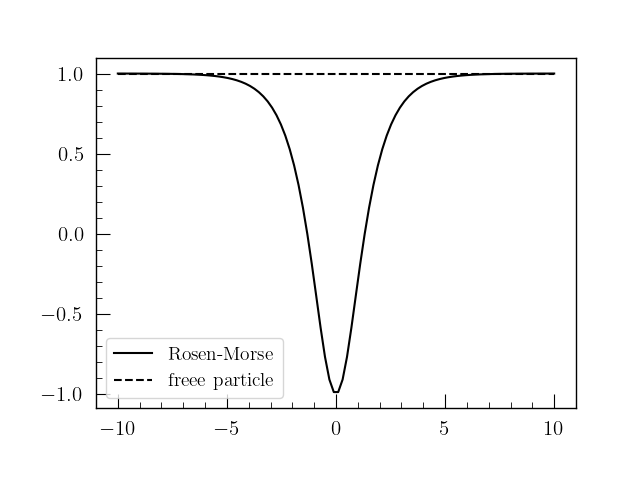
\includegraphics[width=6cm]{./potentials/free-RM.png}
					\caption{自由粒子とRosen--Morseポテンシャルの比較.}
					\label{fig:Rosen-Morse}
				\end{minipage}&
				\begin{minipage}[t]{0.45\hsize}
					\centering
					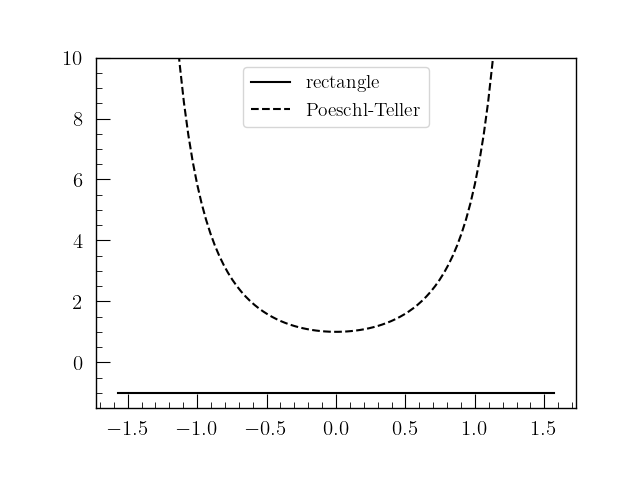
\includegraphics[width=6cm]{./potentials/rectangle-PT.png}
					\caption{井戸型ポテンシャルとP\"{o}schl--Tellerポテンシャルの比較.}
					\label{fig:Poeschl-Teller}
				\end{minipage}
			\end{tabular}
		\end{figure}

	\section{Exactly solvable model}
	\begin{defn}[Exactly solvable]
		Exactly solvableとは,量子力学系のエネルギー固有値と固有関数がすべてわかることを指す.
	\end{defn}
	
	\begin{thm}\label{thm:construct_by_groundstate}
		一次元量子力学系でground state $\psi_0(x)$とground energy $E_0$が与えられているとする.
		このとき,
		\begin{align}
			W'(x) &\coloneqq -\hbar \psi_0(x)/\psi_0(x)\label{eq:Wp_solv}\\
			A & \coloneqq -\frac{\i\hbar}{\sqrt{2m}}\qty(\dv{}{x} + \frac{1}{\hbar}W'(x))\label{eq:A_solv}\\
			A^{\dag} &= -\frac{\i\hbar}{\sqrt{2m}}\qty(\dv{}{x} - \frac{1}{\hbar}W'(x))
		\end{align}
		とすると,Hamiltonianは$H = A^{\dag}A + E_0$となる.

		また,$A\psi_0(x) = 0$を満たす.
	\end{thm}

	量子力学なので,Hamiltonianは$H = -\hbar^2/(2m)\dv*[2]{}{x} + V(x)$である.Ground stateに関して,$H\psi_0(x) = E_0\psi_0(x)$なので,
	\begin{equation}
		V(x) = \frac{\hbar^2}{2m}\frac{\psi_0''(x)}{\psi_0(x)} + E_0
	\end{equation}
	である.
	部分積分をすると,$\hbar^2\psi_0''(x)/\psi_0(x) = -\hbar W''(x) +(W'(x))^2$だから
	\begin{equation}
		V(x) = \frac{1}{2m}W'(x) - \frac{\hbar}{2m}W''(x) + E_0\label{eq:SUSY_potential}
	\end{equation}
	となる.よって,Eq. \eqref{eq:A_solv}のように$A$を設定すれば,$H = A^{\dag}A + E_0$となる.

	また,定義から計算すれば,$A\psi_0(x) = 0$となる.\qed

	Theorem. \ref{thm:construct_by_groundstate}では$W'(x)$を一つ与え,
	Eq. \eqref{eq:SUSY_potential}の形の$V(x)$を求めたが,
	この形のポテンシャルをつくる$W'(x)$がわかれば,同様の手法で解を構成できる.
	次は,ポテンシャル
	\begin{equation}
		V_{(1)}(x) = \frac{1}{2m}(W'(x))^2 -\frac{\hbar}{2m}W''(x)
	\end{equation}
	が与えられたとき,これを$W'(x)$について解いて,他の可解量子力学系を構成する方法を考える.
	この非線形な微分方程式はRiccati型として知られており,
	$\phi(x) \coloneqq \e^{-W(x)/\hbar}$とおくことで,Schr\"{o}dinger型の微分方程式
	\begin{equation}
		-\frac{\hbar^2}{2m}\dv[2]{\phi(x)}{x} + V_{(1)}(x)\phi(x) = \mathcal{E}_{(1)}\phi(x)\label{eq:Riccati_Schroedinger}
	\end{equation}
	に線形化できる.ここで,$\mathcal{E}_{(1)}$は$\mathcal{E}_{(1)} < E_0$を満たす\footnote{$A^{\dag}A$の形にする以上,固有値は必ず非負になる.最低エネルギーが$E_0$にシフトしたので,この場合に非負という条件はこのようになる.}ように取れるパラメータである\footnote{パラメータはこの条件を満たしても,super@otentialの素性が悪くなる(発散したりする)こともあるようである.そうならない範囲でパラメータは自由に取れる.}.
	\begin{thm}
		今,Eq. \eqref{eq:Riccati_Schroedinger}の特解を$\phi_{\S}(x)$を用いて,一般解は
		\begin{equation}
			W_{(1)}'(x) = -\hbar \frac{\phi_{\S}'(x)}{\phi_\S(x)} - \frac{\hbar(\phi_\S(x)^{-2})}{c_{(1)} + \displaystyle\int_{x_0}^{x}\dd{z}(\phi_{\S}(z))^{-2}}
		\end{equation}
		とかける.
	\end{thm}
	$\phi(x)\coloneqq \rho(x)\phi_\S(x)$とする.Eq. \eqref{eq:Riccati_Schroedinger}に代入すると,
	$\rho''(x)\phi_\S(x) + 2\rho'(x)\phi'_\S(x) = 0$を満たすことがわかる.今,$\rho'(x)\phi_\S(x)$でわって,
	\begin{equation}
		\frac{\rho''(x)}{\rho'(x)} + \frac{2\phi_\S'(x)}{\phi_\S(x)} = \dv{}{x} \qty(\log \rho'(x)(\phi_\S(x))^2)
	\end{equation}
	なので,
	\begin{equation}
		\rho(x) = c_1 + \int_{x_0}^{x}\dd{z}c_0(\phi_\S(x))^{-2}
	\end{equation}
	となる.$c_0$, $c_1$は積分定数である.

	定義をたどって,元に戻すと,
	\begin{equation}
		W'(x) = - \hbar\frac{\phi'_\S(x)}{\phi_\S(x)} - \frac{\hbar(\phi_\S(x))^{-2}}{c_1/c_0 + \int_{x_0}^{x}\dd{z}(\phi_\S(z))^{-2}}
	\end{equation}
	となり,$c_{(1)} = c_1/c_0$と置くことで示せる.\qed


	以上より求まった,$W'_{(1)}(x)$を用いて,$A_{(1)}$を定めることでHamiltonianは$H_{(1)} = A_{(1)}^\dag A_{(1)} + \mathcal{E}_{(1)}$となり,エネルギースペクトラムが同じの超対称パートナーは
	$H_{(2)} = A_{(1)}A_{(1)}^{\dag} + \mathcal{E}_{(1)}$となる.$H_{(1)}$がexactly solvableなら$H_{(2)}$についても完全にわかったことになる.
	また,$H_{(2)}$も量子力学のHamiltonianなので,$H_{(2)} = A_{(2)}^{\dag}A_{(2)} + \mathcal{E}_{(1)} + \mathcal{E}_{(1)}$とできる.ここから$H_{(3)}$が作れるなど,この操作を繰り返したくさんの可解量子力学系のfamilyを作ることができる.
\end{document}

\end{document}
